\begin{subsectionframemod}{Few-Shot Object Detection}
    \metroset{block=fill}
    \vspace{-10mm}
    \begin{alertblock}{Détection d'objets $n$-way $k$-shot}
        Étant donné des exemples de support $\{(x_1, a_1), \dots, (x_{nk}, a_{nk})\}$, il s'agit de détecter toutes les occurrences des classes dans $\mathcal{C}$ ($|\mathcal{C}| = n$) dans une image de requête $x_q$.
        En règle générale, $k$ est compris entre 1 et 50.
    \end{alertblock}

    \vspace{5mm}
    \pause
    \begin{columns}
        \begin{column}{0.3\textwidth}
            \centering
            \begin{tikzpicture}
                \node[anchor=south west,inner sep=0, label=below:{\small Query image}] at (0,0){
                    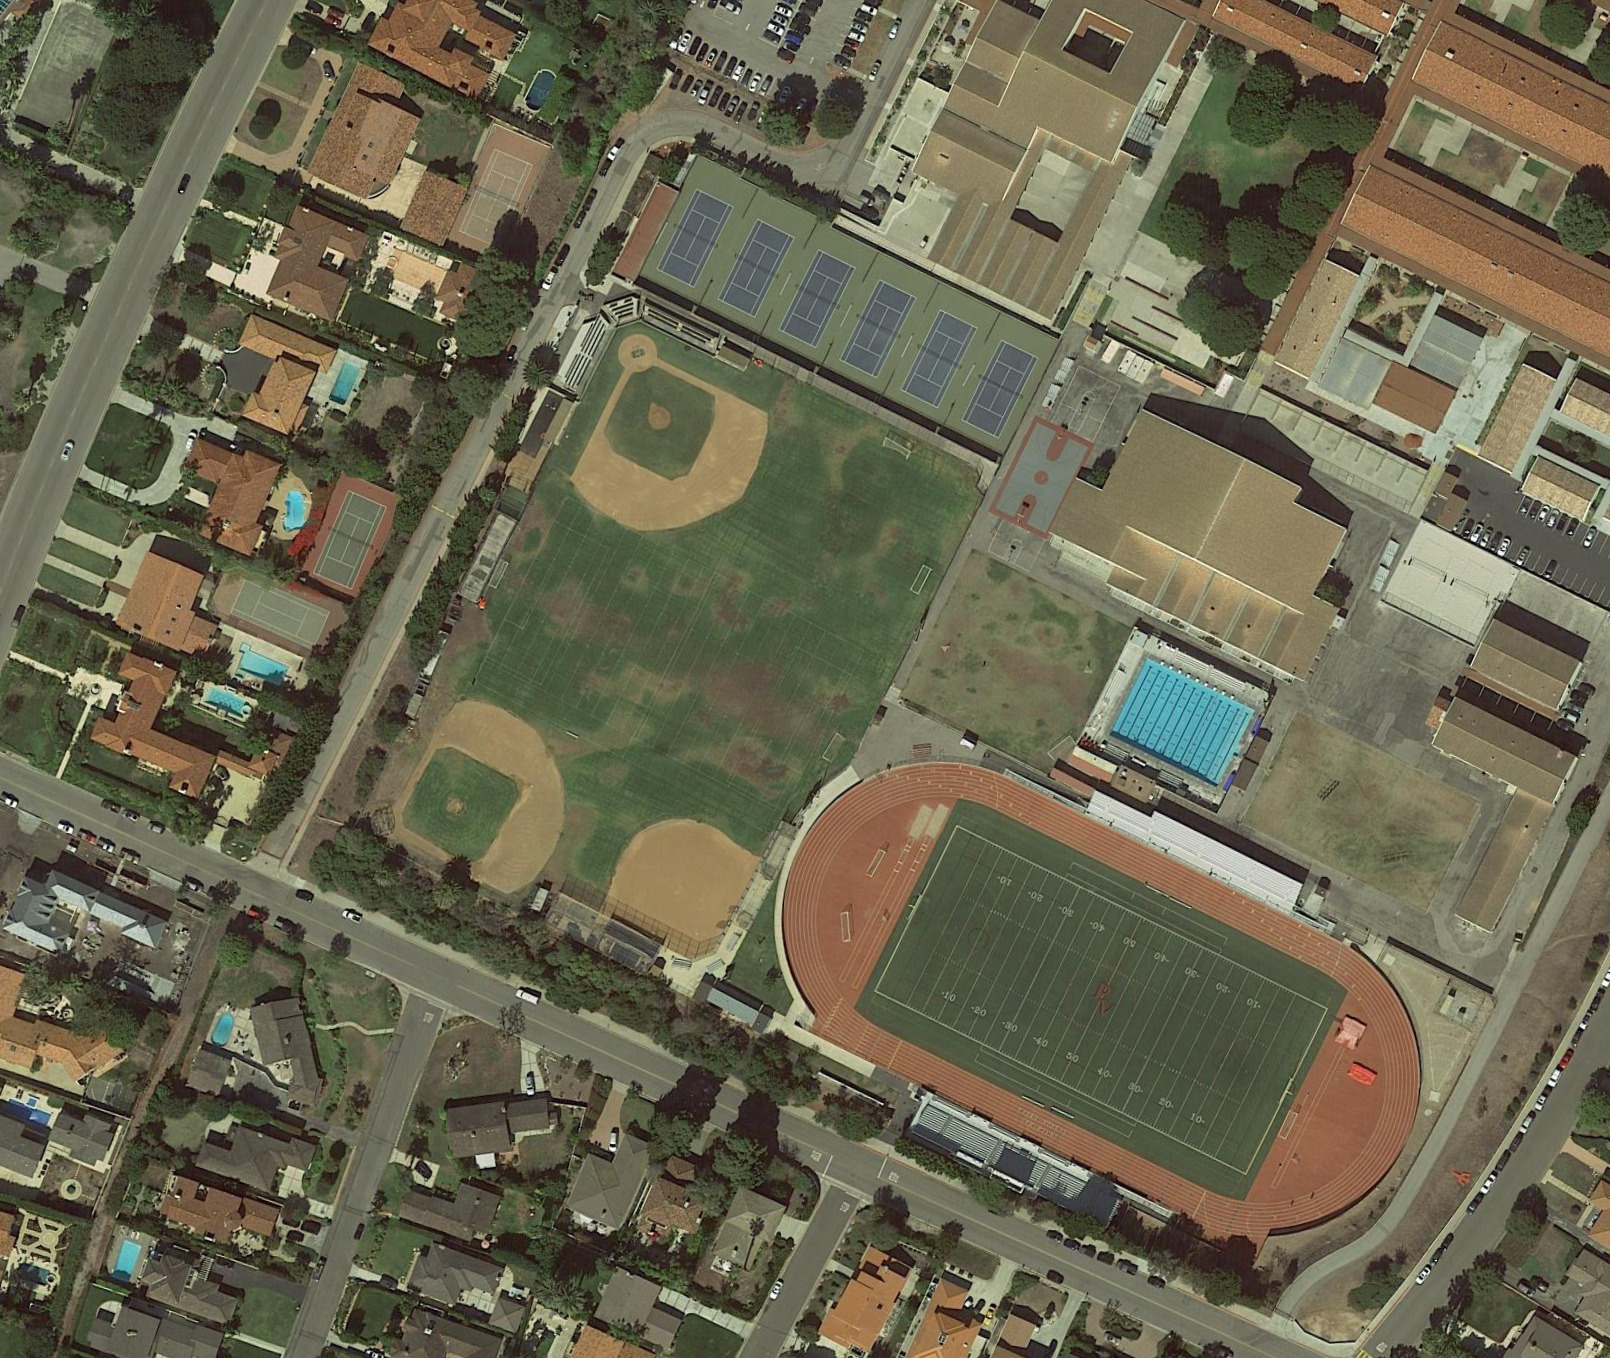
\includegraphics[width=30mm]{Figures/P0770}
                };
               
            \end{tikzpicture}
            
        \end{column}
        \pause
        
        \begin{column}{0.3\textwidth}
            
            \begin{tikzpicture}[remember picture,overlay]
                \only<3->{
                    \node[xshift=\paperwidth/2,yshift=-\paperheight/2-32mm, label=below:{\small $n$ classes, $k$ images par classes}](support) at (current page.north west){%

                    \graphicsbox{Figures/P0131.jpg}{(0.2,0.2)}{(0.23,0.5)}{green}[15mm][0.2mm]
                    \graphicsbox{Figures/P0168.jpg}{(0.26,0.38)}{(0.07,0.07)}{blue}[15mm][0.2mm]
                    \graphicsbox{Figures/P0352.jpg}{(0.6,0.18)}{(0.3,0.3)}{red}[15mm][0.2mm]
                    };
                }
                
                
                \only<4->{\draw[decorate, decoration ={brace,raise=1pt}] (support.north west) -- (support.north east)
                    node (supportlabel) [midway, above=10pt] {\huge $\uparrow$};}

            \end{tikzpicture}
            \only<4->{
                \begin{textblock*}{50mm}(41mm,53mm)
                    \huge $\rightarrow$
                \end{textblock*}
                

                \begin{tikzpicture}[remember picture,overlay]
                    \node[xshift=\paperwidth/2 +0mm,yshift=-\paperheight/2- 5.5mm] at (current page.north west){%
                        \fbox{\parbox[][10mm][c]{0.8\textwidth}{\centering\normalsize Modèle de détection few-shot}}
                    };
                \end{tikzpicture}
            }
            % \graphicsbox{Figures/P0131.jpg}{(0.2,0.2)}{(0.23,0.5)}{green}[20mm][0.2mm]
        \end{column}
        \pause
        \begin{column}{0.3\textwidth}
            \only<5->{
                \begin{textblock*}{50mm}(82mm,53mm)
                    \huge $\rightarrow$
                \end{textblock*}
                \centering
                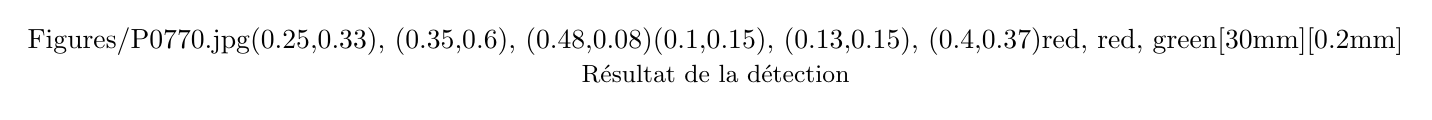
\begin{tikzpicture}
                    \node[anchor=south west,inner sep=0, label=below:{\small Résultat de la détection}] at (0,0){
                        \graphicsbox{Figures/P0770.jpg}{(0.25,0.33), (0.35,0.6), (0.48,0.08)}{(0.1,0.15), (0.13,0.15), (0.4,0.37)}{red, red, green}[30mm][0.2mm]
                    };
                
                \end{tikzpicture}
            }
            
        \end{column}
    \end{columns}
        
\end{subsectionframemod}